% =====================================================================
%  Introduction to Deep Learning — Class 18
%  Topic (course plan): Deep Networks
%  Subtopic (course plan): Regularization: Explicit and Implicit
%  Sources (course plan): Prince Chapter 9, Bishop Chapter 9
%
%  Class 17 ended with the fact that past the interpolation threshold
%  many parameter vectors fit the data equally well, so the test error
%  is decided by WHICH one the procedure returns.  This class is about
%  that choice: first the preference we write into the objective, then
%  the one the optimiser already has without being asked.
%
%  Order: why a preference is unavoidable, the penalty and what it does
%  to each eigen-direction, the shape of the penalty, then the implicit
%  preference of GD and SGD, then bias built into the architecture.
%
%  Heuristics, early stopping, dropout and augmentation are Class 19.
%
%  C variant: the B deck with the one result absent from both set texts
%  removed -- the eigenbasis shrinkage factor and the effective-parameter
%  count, which Bishop (2024) describes only qualitatively and attributes
%  to Bishop (2006) and Hastie et al. (2009).  Two slides go with it.
%  See _shared/PLAN_Classes17_18_19.md.
%
%  Compile:  xelatex main.tex   (run twice)
% =====================================================================
\documentclass[aspectratio=169, 11pt]{beamer}

\usetheme{metropoliscustom}

\usepackage{graphicx}
\DeclareGraphicsExtensions{.pdf,.png,.jpg}
\graphicspath{{figs/}{Class18_Regularization_Explicit_Implicit/C_Textbook_Theorems_Only/figs/}}
\usepackage{amsmath, amssymb}
\usepackage{bm}
\usepackage{tikz}
\usetikzlibrary{arrows.meta, positioning, calc, decorations.pathreplacing,
                shapes.geometric, fit, backgrounds}
\tcbuselibrary{skins}

\definecolor{shc}{HTML}{341651}
\definecolor{tealc}{HTML}{1C7293}
\definecolor{dpc}{HTML}{800000}
\definecolor{accc}{HTML}{B8860B}

% ---- theorem environments -------------------------------------------
\setbeamertemplate{theorems}[numbered]
\usepackage{remreset}
\makeatletter\@removefromreset{theorem}{section}\makeatother
\renewcommand{\thetheorem}{\arabic{theorem}}
\newtheorem{lemmax}[theorem]{Lemma}
\newtheorem{propx}[theorem]{Proposition}
\newtheorem{corx}[theorem]{Corollary}
\newtheorem{defx}[theorem]{Definition}
\newtheorem{thmx}[theorem]{Theorem}

\newcommand{\bridge}[1]{%
  {\scriptsize\itshape\color{mcMuted} #1\par}\vspace{0.35em}}

\newcommand{\srcline}[1]{%
  \par\vspace{0.25em}%
  {\scriptsize\color{mcMuted}\hfill #1\par}}

\newcommand{\figsource}[1]{{\scriptsize\color{mcMuted} #1}}
\newcommand{\figcap}[2][0.90]{%
  \begin{center}\begin{minipage}{#1\textwidth}\centering
    {\scriptsize\color{mcMuted} #2}
  \end{minipage}\end{center}}

% =====================================================================
\title{Deep Networks}
\subtitle{Regularization: Explicit and Implicit}
\author{Introduction to Deep Learning \ \textperiodcentered\ Class 18}
\institute{}
\date{}

\footleft{Introduction to Deep Learning}
\footright{Explicit and Implicit Regularization}
\titlelogos{}

\begin{document}

\maketitle

\begin{frame}{Outline}
  \tableofcontents
\end{frame}

% =====================================================================
\section{Why a Preference Is Unavoidable}
% =====================================================================

\begin{frame}{From measuring the error to choosing the solution}
  \bridge{Class 17 ended with the fact that past the interpolation
  threshold many parameter vectors fit the data equally well, and the
  test error is decided by which one the procedure returns.}
  \vspace{0.35em}
  {\footnotesize
  \renewcommand{\arraystretch}{1.36}
  \begin{tabular}{@{}l@{\hspace{1.6em}}l@{}}
    \textbf{Settled in Class 17} & \textbf{Open today}\\
    error $=$ bias$^2 +$ variance $+$ noise & how to move the
      bias--variance balance on purpose\\
    many exact fits exist above the threshold & which of them the
      procedure returns, and why\\
    smooth interpolants generalize better & what makes a procedure
      prefer one\\
  \end{tabular}}
  \vspace{0.9em}

  \begin{redhighlight}
    Two mechanisms: a term we add to the objective, and a preference the
    optimiser already has without being asked.
  \end{redhighlight}
\end{frame}

\begin{frame}{Notation for today}
  \vspace{0.4em}
  {\footnotesize
  \renewcommand{\arraystretch}{1.34}
  \begin{columns}[T, onlytextwidth]
    \begin{column}{0.49\textwidth}
      \begin{tabular}{@{}l@{\hspace{1.5em}}l@{}}
        $E(\mathbf{w})$ & the training error of Class 13\\
        $\Omega(\mathbf{w})$ & the regularization term\\
        $\lambda$, $\alpha$ & its coefficient\\
        $\widetilde{E}(\mathbf{w})$ & $E(\mathbf{w}) + \lambda\,\Omega(\mathbf{w})$\\
      \end{tabular}
    \end{column}
    \begin{column}{0.49\textwidth}
      \begin{tabular}{@{}l@{\hspace{1.5em}}l@{}}
        $\lambda_i$, $\mathbf{u}_i$ & eigenvalues and eigenvectors of $\mathbf{H}$\\
        $\eta$ & the step size, as in Class 13\\
        $\widetilde{L}$ & the \emph{modified} loss of an optimiser\\
        $B$ & number of batches in an epoch\\
      \end{tabular}
    \end{column}
  \end{columns}}
  \vspace{0.6em}

  \begin{itemize}\itemsep0.28em
    \item Bishop writes the penalty coefficient $\lambda$ and Prince
          writes it $\lambda$ too; Bishop's $\alpha$ appears when the
          penalty is read as a prior precision
    \item $\mathbf{H}$ and its eigen-decomposition are the ones from Class 13
  \end{itemize}
  \srcline{Bishop \& Bishop (2024), Eq.~9.1; Prince (2023), Eq.~9.2.}
\end{frame}

\begin{frame}{Learning from data alone is not possible}
  \vspace{-0.1em}
  \begin{propx}[No free lunch]\label{th:nfl}
    \small
    Averaged over all possible problems, every learning algorithm
    performs equally well: one that beats the average on some problems
    must fall below it on others.
  \end{propx}
  \vspace{0.15em}
  \begin{itemize}\itemsep0.24em
    \item So no algorithm is universally best, and the useful question
          is which problems an algorithm is \alert{biased towards}
    \item The space of all problems includes relations no application
          would ever produce; real ones are mostly smooth, and most
          models are biased towards smoothness
    \item A finite parameter count is itself a bias; there is no
          unbiased option
  \end{itemize}
  \vspace{-0.35em}
  \srcline{Wolpert (1996); Bishop \& Bishop (2024), \S9.1.2.}
\end{frame}

\begin{frame}{The data does not determine the function}
  \begin{center}
    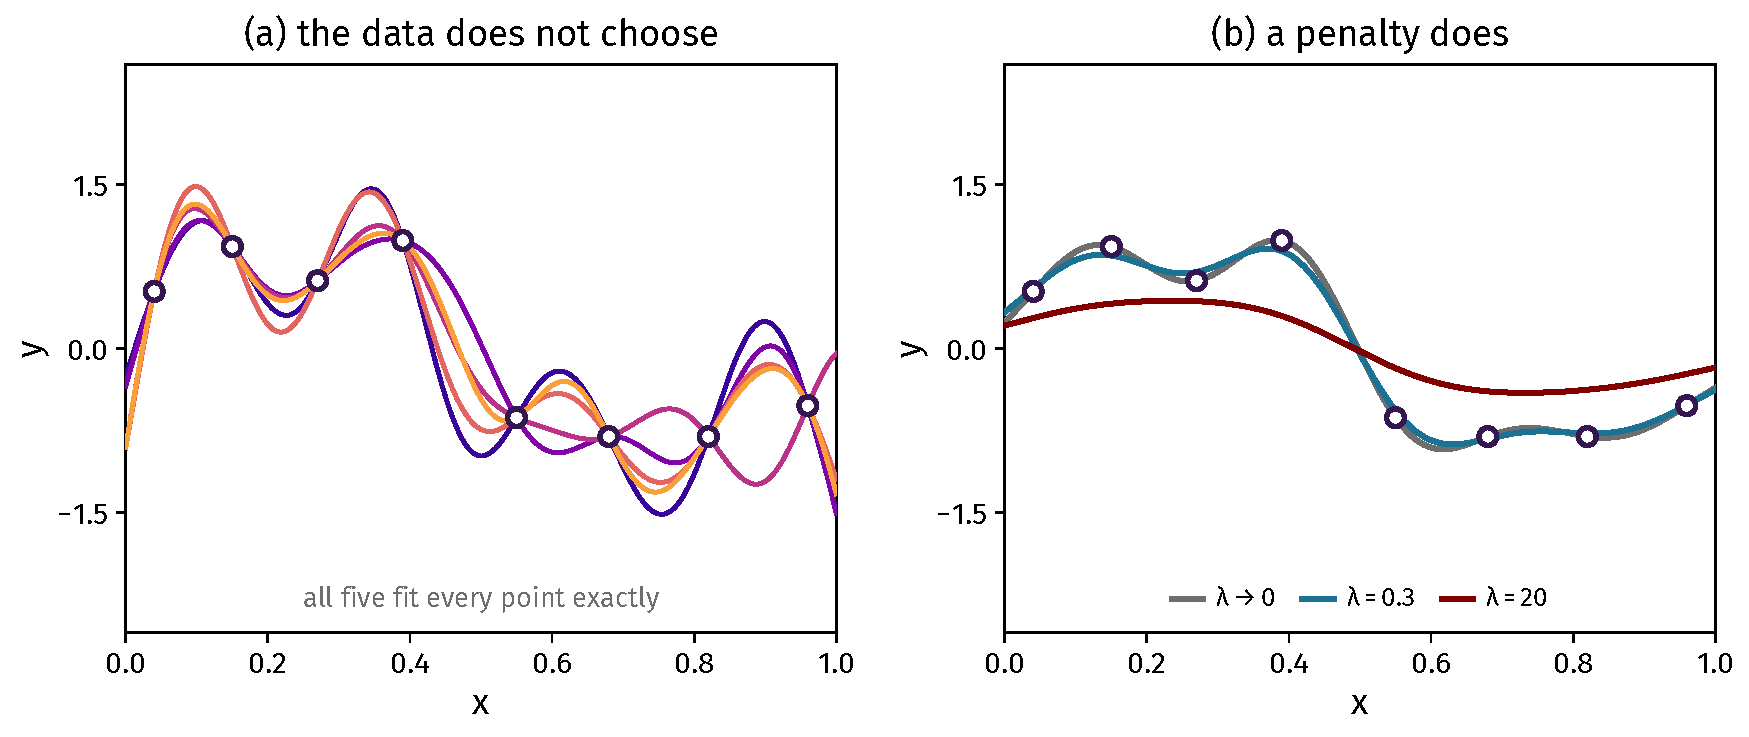
\includegraphics[width=0.735\linewidth]{underdetermined}
  \end{center}
  \figcap[0.97]{(a) five functions, each through all eight observations:
  the training error cannot separate them. (b) a penalty on the weights
  singles one out, and its coefficient decides which.}
  \srcline{Bishop \& Bishop (2024), \S9.1.1.}
\end{frame}

\begin{frame}{A penalty reshapes the whole surface}
  \begin{center}
    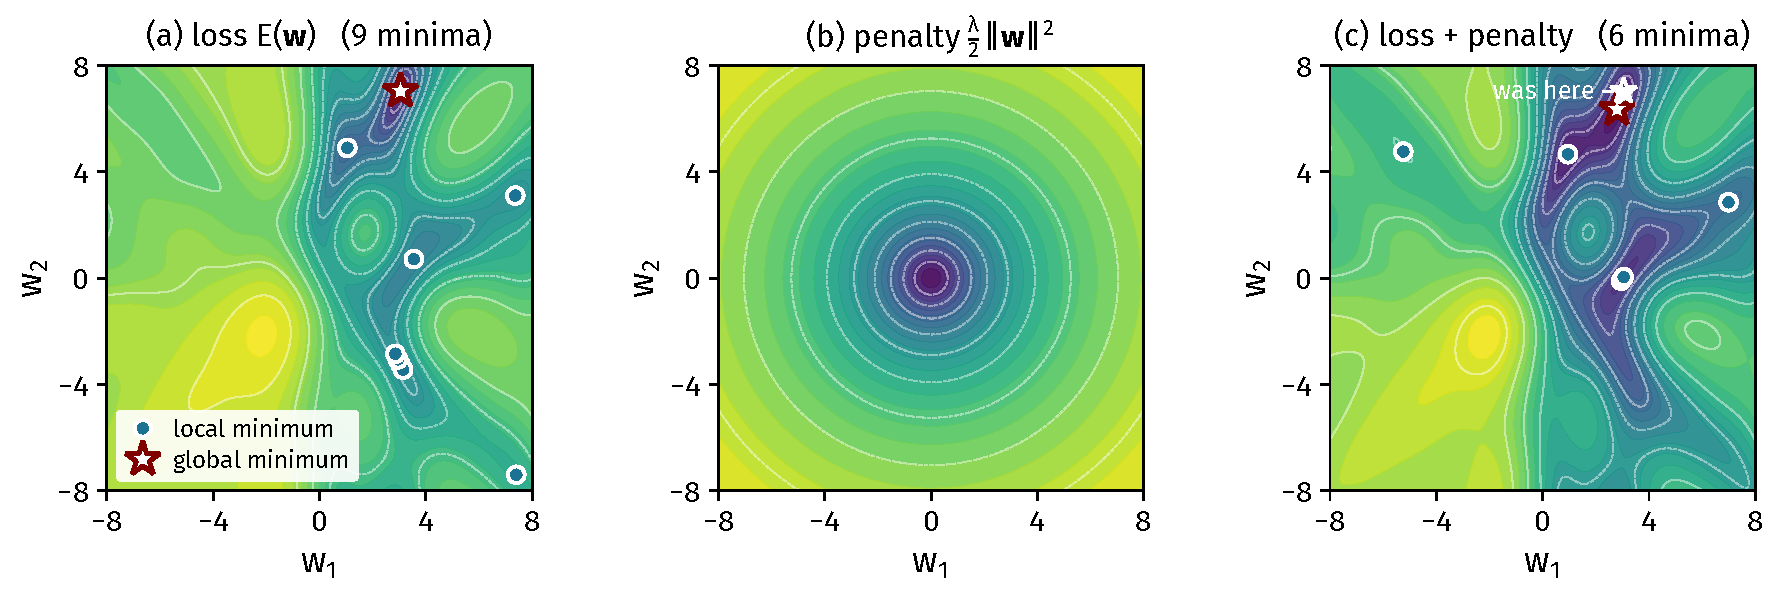
\includegraphics[width=0.82\linewidth]{loss_regularization}
  \end{center}
  \vspace{-0.2em}
  \figcap[0.97]{$\hat y = \sin(w_1 x) + \tfrac12 \sin(w_2 x)$ on $40$
  points. (a) the loss: nine local minima (dots), one global (star).
  (b) the penalty $\tfrac{\lambda}{2}\|\mathbf{w}\|^2$. (c) their sum: six
  minima remain, and the global one has moved towards the origin.}
  \srcline{Prince (2023), \S9.1, Fig.~9.1.}
\end{frame}

\begin{frame}{Three places to put a preference}
  \vspace{0.3em}
  {\footnotesize
  \renewcommand{\arraystretch}{1.42}
  \begin{tabular}{@{}l@{\hspace{1.2em}}l@{\hspace{1.2em}}l@{}}
    \textbf{Where} & \textbf{Example} & \textbf{Covered}\\
    the model class & basis functions, depth, weight sharing & today\\
    the objective & $\lambda\|\mathbf{w}\|^2$, the lasso & today\\
    the algorithm & the step size, the batch size & today\\
    the data & augmentation, added noise & Class 19\\
    the stopping rule & early stopping & Class 19\\
  \end{tabular}}
  \vspace{0.65em}

  \begin{redhighlight}
    The first three are properties of the model and the optimiser and
    apply before a single epoch is run. The last two are things done to
    the training procedure, and are the subject of the next class.
  \end{redhighlight}
\end{frame}

% =====================================================================
\section{Explicit Regularization}
% =====================================================================

\begin{frame}{The regularized objective}
  \vspace{-0.2em}
  \[
    \hat{\mathbf{w}} \;=\; \arg\min_{\mathbf{w}}
      \Big[\, \underbrace{\textstyle\sum_{n} \ell_n(\mathbf{w})}_{\text{fit}}
        \;+\; \lambda\, \underbrace{\Omega(\mathbf{w})}_{\text{preference}} \Big],
    \qquad
    \Omega(\mathbf{w}) = \tfrac12 \|\mathbf{w}\|^2 .
  \]
  \vspace{-0.5em}
  \begin{itemize}\itemsep0.32em
    \item $\Omega$ returns a larger value for parameters we like less;
          $\lambda$ sets how much that opinion counts
    \item The minima of $\widetilde{E}$ are not the minima of $E$, so
          training converges somewhere else on purpose
    \item For the quadratic choice the gradient is
          $\nabla \widetilde{E} = \nabla E + \lambda\mathbf{w}$, which is why it
          is called \alert{weight decay}: each step pulls $\mathbf{w}$ towards
          the origin
  \end{itemize}
  \srcline{Bishop \& Bishop (2024), Eqs.~9.1, 9.5; Prince (2023), Eq.~9.2.}
\end{frame}

\begin{frame}{The penalty is a prior}
  \vspace{-0.15em}
  \begin{propx}[Maximum a posteriori]\label{th:map}
    \small
    Maximising the posterior
    $\prod_n p(Y_n \mid \mathbf{x}_n, \mathbf{w})\, p(\mathbf{w})$
    is the same as minimising
    $\sum_n \ell_n(\mathbf{w}) + \lambda\,\Omega(\mathbf{w})$
    with
    \[
      \lambda\,\Omega(\mathbf{w}) \;=\; -\log p(\mathbf{w}),
    \]
    so a quadratic penalty is a zero-mean Gaussian prior of precision
    $\lambda$, and the lasso is a Laplace prior.
  \end{propx}
  \vspace{0.3em}
  \begin{itemize}\itemsep0.28em
    \item Choosing a penalty is choosing what we believed before seeing
          any data
    \item The awkwardness is that the belief is expressed over
          \emph{parameters}, while what we actually know concerns the
          \emph{function}
  \end{itemize}
  \srcline{Prince (2023), \S9.1.1, Eqs.~9.3--9.4; Bishop \& Bishop (2024), \S9.2.}
\end{frame}

\begin{frame}{Weight decay, drawn}
  \vspace{-0.3em}
  \begin{center}
    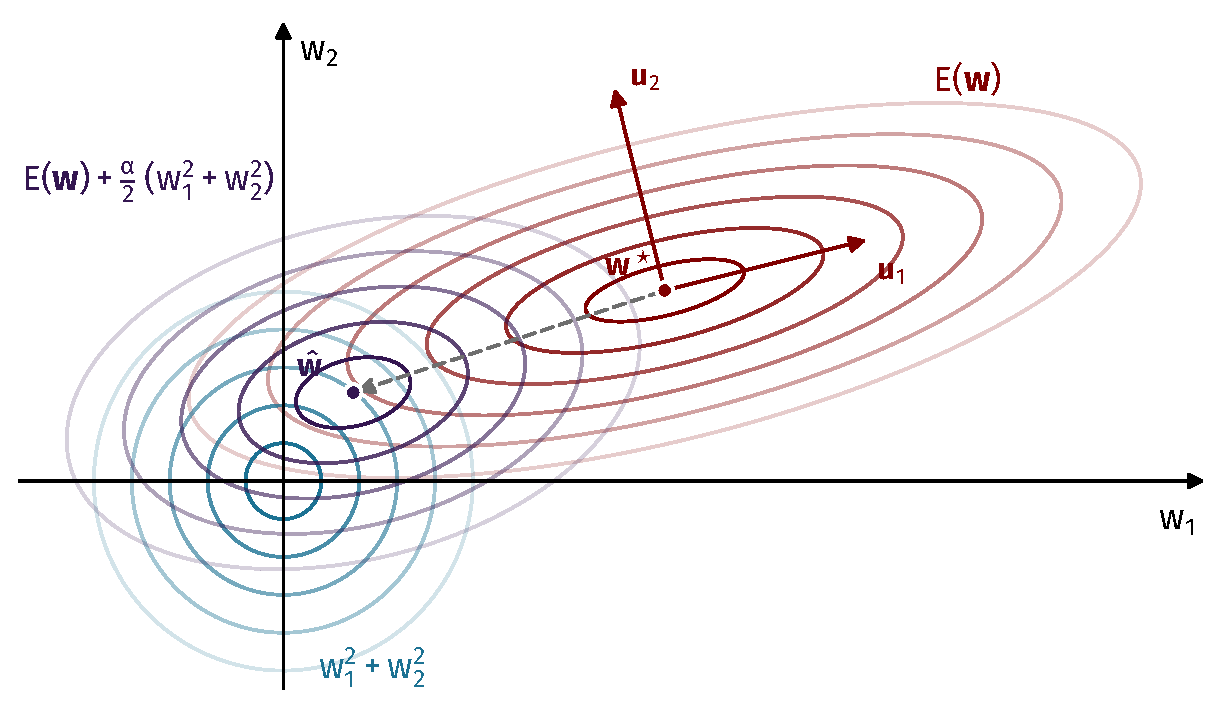
\includegraphics[width=0.56\linewidth]{weight_decay_geometry}
  \end{center}
  \vspace{-0.4em}
  \figcap[0.97]{Contours of the error (maroon), the penalty (teal) and
  their sum (indigo), axes $\mathbf{u}_i$ of the Hessian drawn at
  $\mathbf{w}^\star$. The minimum moves $2.32$ along $\mathbf{u}_1$, where
  the error is insensitive, and $0.17$ along $\mathbf{u}_2$.}
  \srcline{Bishop \& Bishop (2024), Fig.~9.3.}
\end{frame}

\begin{frame}{What the coefficient costs}
  \begin{center}
    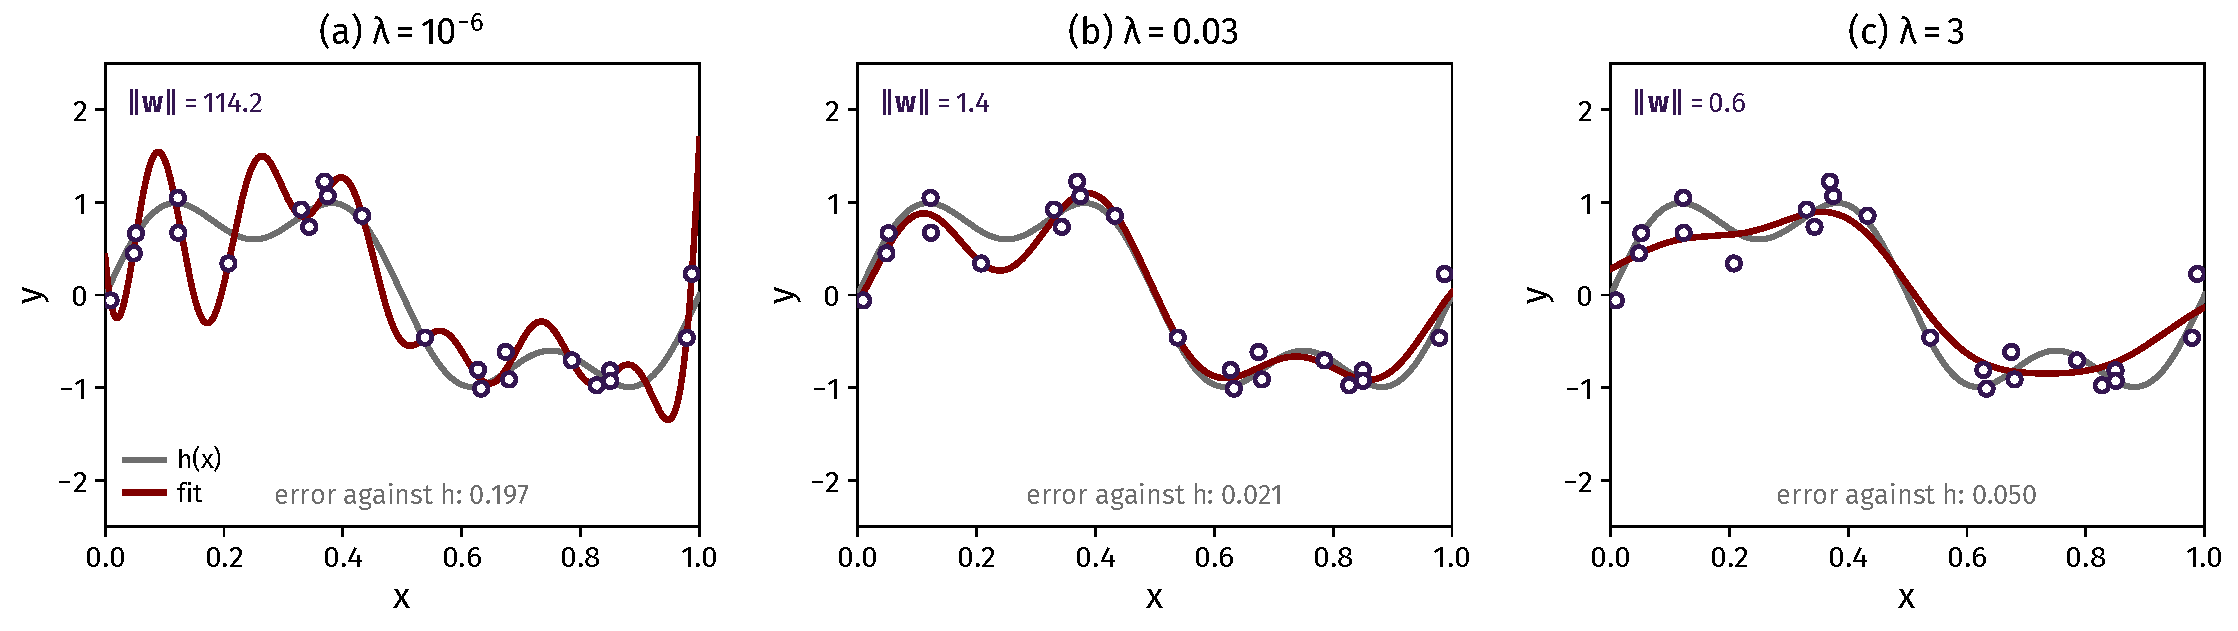
\includegraphics[width=0.94\linewidth]{penalty_sweep}
  \end{center}
  \figcap[0.97]{The same $45$-parameter model on the same $22$ points.
  The weight norm falls from $114$ to $0.6$; the error against $h$ falls
  from $0.197$ to $0.021$ and then rises to $0.050$.}
  \srcline{Prince (2023), Fig.~9.2.}
\end{frame}

\begin{frame}{A regularizer should respect the model's symmetries}
  \vspace{-0.2em}
  \begin{propx}[Consistent regularizers]\label{th:consist}
    \small
    Rescaling the inputs, $x_i \to a x_i + b$, leaves the network
    function unchanged provided the first-layer weights transform as
    $w_{ji} \to w_{ji}/a$, and similarly for the outputs. Simple weight
    decay is \emph{not} invariant under this, but the layer-wise
    regularizer
    \[
      \frac{\lambda_1}{2}\sum_{w \in \mathcal{W}_1} w^2
      \;+\; \frac{\lambda_2}{2}\sum_{w \in \mathcal{W}_2} w^2 ,
      \qquad \text{biases excluded,}
    \]
    is, provided $\lambda_1 \to a^{1/2}\lambda_1$ and
    $\lambda_2 \to c^{-1/2}\lambda_2$.
  \end{propx}
  \vspace{0.1em}
  \begin{itemize}\itemsep0.22em
    \item Otherwise changing the units of a feature would change which
          solution we prefer, which is not a preference about the world
  \end{itemize}
  \srcline{Bishop \& Bishop (2024), Eqs.~9.6--9.15.}
\end{frame}

\begin{frame}{Other shapes of penalty}
  \vspace{-0.2em}
  \[
    \Omega(\mathbf{w}) \;=\; \frac{1}{2}\sum_{j=1}^{W} |w_j|^q ,
    \qquad
    \text{equivalently} \quad
    \min_{\mathbf{w}} E(\mathbf{w}) \ \ \text{subject to} \ \
    \sum_{j=1}^{W} |w_j|^q \leq \eta .
  \]
  \vspace{-0.6em}
  \begin{center}
    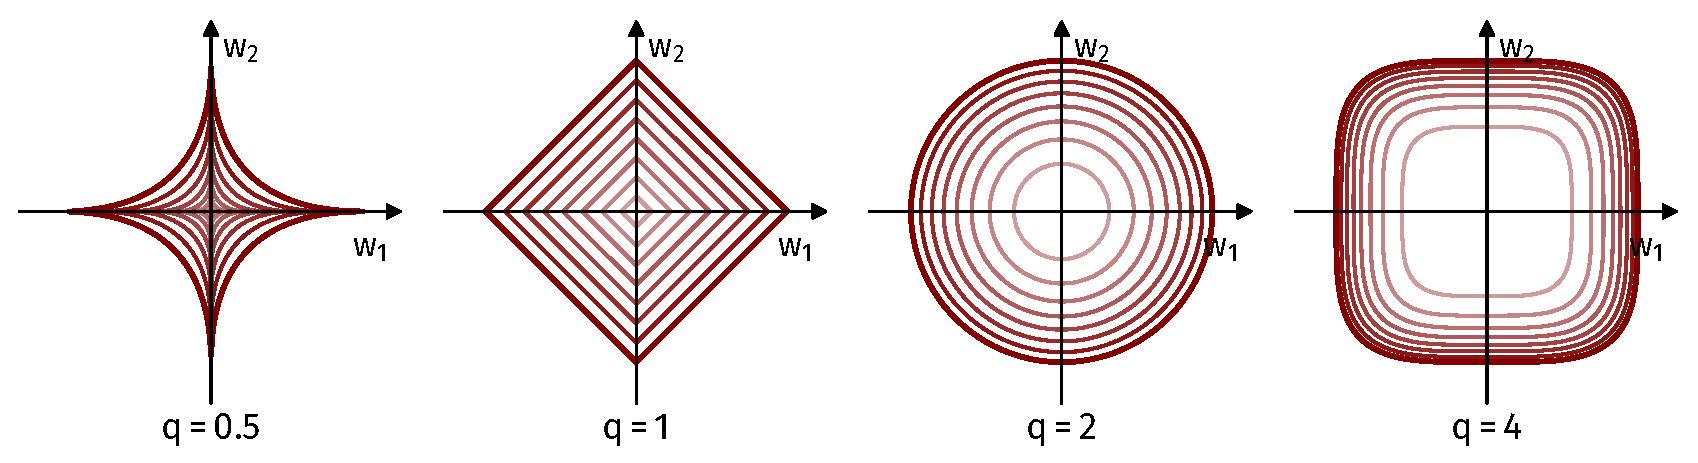
\includegraphics[width=0.60\linewidth]{qnorm_contours}
  \end{center}
  \vspace{-0.55em}
  \figcap[0.97]{Level sets of the penalty. Only $q \leq 1$ has corners
  on the axes; only $q \geq 1$ is convex; $q = 1$ alone has both, and
  is the lasso.}
  \srcline{Bishop \& Bishop (2024), Eqs.~9.18--9.20, Fig.~9.5.}
\end{frame}

\begin{frame}{Why the lasso sets coefficients to zero}
  \vspace{-0.15em}
  \begin{propx}[Sparsity from corners]\label{th:lasso}
    \small
    In the constrained form the solution lies where a contour of $E$
    first touches the region $\sum_j |w_j|^q \leq \eta$. For $q = 1$
    that region is a polytope whose vertices lie on the coordinate axes,
    so for a generic error function contact occurs at a vertex and some
    coordinates are \alert{exactly} zero. For $q = 2$ the boundary is
    smooth and has no such points.
  \end{propx}
  \vspace{0.3em}
  \begin{itemize}\itemsep0.26em
    \item Increasing $\lambda$, equivalently shrinking $\eta$, drives
          more coefficients to zero and the corresponding basis
          functions out of the model
    \item Weight decay shrinks the same coefficients but never reaches
          zero
  \end{itemize}
  \srcline{Tibshirani (1996); Bishop \& Bishop (2024), \S9.2.2, Fig.~9.6.}
\end{frame}

\begin{frame}{The two geometries side by side}
  \vspace{-0.3em}
  \begin{center}
    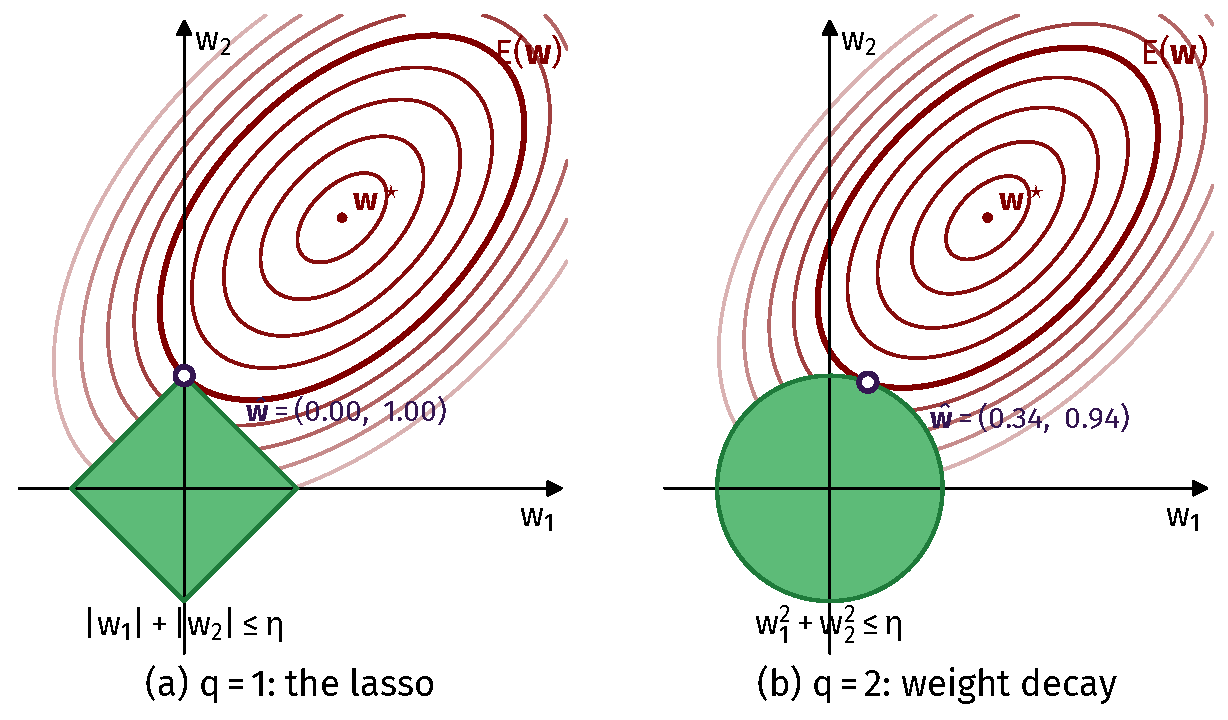
\includegraphics[width=0.49\linewidth]{lasso_vs_ridge}
  \end{center}
  \vspace{-0.4em}
  \figcap[0.97]{Error contours (maroon) and constraint region (green),
  same $E$ and same $\eta$. (a) the lasso makes contact at a vertex, so
  $\hat w_1 = 0$ exactly. (b) the quadratic penalty makes contact on a
  smooth arc and merely reduces it, to $0.34$.}
  \srcline{Bishop \& Bishop (2024), Fig.~9.6.}
\end{frame}

% =====================================================================
\section{Implicit Regularization}
% =====================================================================

\begin{frame}{The optimiser has a preference too}
  \vspace{0.2em}
  \begin{itemize}\itemsep0.38em
    \item Nothing so far explains why an unregularized network, trained
          to zero training error, generalizes at all
    \item On a surface with a whole valley of global minima, the loss is
          equal everywhere along it, so \alert{only the algorithm} can
          decide where to stop
    \item Gradient descent does not move neutrally: the discretisation
          itself expresses a preference, and so does the sampling of
          batches
    \item Both preferences can be written down as extra terms in a
          modified loss, and both can be checked
  \end{itemize}
  \srcline{Prince (2023), \S9.2.}
\end{frame}

\begin{frame}{What the step size is really minimising}
  \vspace{-0.25em}
  \begin{thmx}[Implicit regularization of gradient descent]\label{th:igd}
    \small
    Continuous gradient flow follows
    $\partial \mathbf{w} / \partial t = -\nabla L(\mathbf{w})$. Discrete descent
    $\mathbf{w}^{(\tau)} = \mathbf{w}^{(\tau-1)} - \alpha \nabla L$ instead follows,
    to leading order in $\alpha$, the flow of the \alert{modified} loss
    \[
      \widetilde{L}_{\mathrm{GD}}(\mathbf{w})
        \;=\; L(\mathbf{w}) \;+\; \frac{\alpha}{4}\,
              \big\| \nabla L(\mathbf{w}) \big\|^2 .
    \]
  \end{thmx}
  \vspace{0.05em}
  {\footnotesize
  \begin{itemize}\itemsep0.22em
    \item The extra term is a penalty on \alert{steepness}: the
          trajectory is pushed away from places where the surface is
          sharp
    \item It vanishes at any stationary point, so it moves the path, not
          the set of minima
    \item Larger $\alpha$ means a stronger penalty --- the step size is
          a regularization coefficient
  \end{itemize}}
  \srcline{Prince (2023), Eq.~9.8; Barrett \& Dherin (2021).}
\end{frame}

\begin{frame}{Where the extra term comes from}
  \vspace{-0.25em}
  {\footnotesize
  \begin{itemize}\itemsep0.30em
    \item \focus{1}{Expand one discrete step to second order:
          $\mathbf{w} - \alpha\nabla L$ differs from the flow evaluated at time
          $\alpha$ by a term of order $\alpha^2$.}
    \item \focus{2}{Along the flow, $\nabla L$ itself changes at rate
          $-\mathbf{H}\nabla L$, so the flow's own second-order term carries
          $+\tfrac{\alpha^2}{2}\mathbf{H}\nabla L$.}
    \item \focus{3}{The discrete step has no such term, so the two
          disagree at order $\alpha^2$ by exactly
          $\tfrac{\alpha^2}{2}\mathbf{H}\nabla L$.}
    \item \focus{4}{Ask which modified loss would reproduce that:
          we need $\nabla \widetilde{L} = \nabla L +
          \tfrac{\alpha}{2}\mathbf{H}\nabla L$.}
    \item \focus{5}{That is a gradient, of
          $L + \tfrac{\alpha}{4}\|\nabla L\|^2$, since
          $\nabla \tfrac12\|\nabla L\|^2 = \mathbf{H}\nabla L$.
          \hfill $\square$}
  \end{itemize}}
  \vspace{-0.2em}
  \begin{redhighlight}
    The penalty is not put there by anyone. It is the price of taking
    steps of finite length instead of following the curve.
  \end{redhighlight}
\end{frame}

\begin{frame}{Testing the claim}
  \begin{center}
    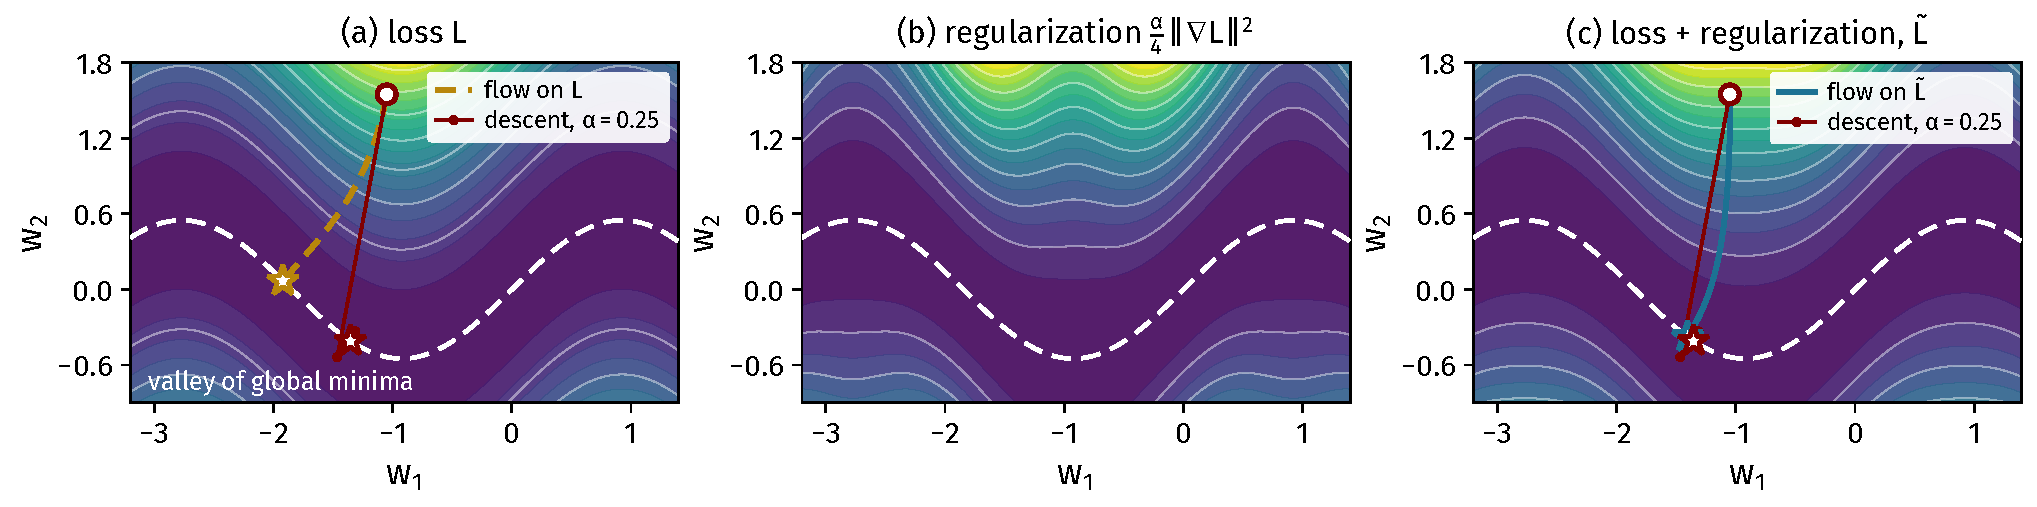
\includegraphics[width=0.90\linewidth]{implicit_gd}
  \end{center}
  \vspace{-0.2em}
  \figcap[0.97]{Every point of the dashed valley is a global minimum.
  (a) the flow on $L$ and discrete descent with $\alpha = 0.25$ reach
  different points of it. (b) the penalty on the squared gradient, zero
  on the floor. (c) with it added, the flow arrives where descent did;
  its endpoint error falls like $\alpha^{1.9}$, the plain flow's like
  $\alpha^{1.0}$.}
  \srcline{Prince (2023), Fig.~9.3.}
\end{frame}

\begin{frame}{What sampling batches adds}
  \vspace{-0.3em}
  \begin{thmx}[Implicit regularization of SGD]\label{th:isgd}
    \small
    Averaging over the possible orderings of $B$ batches, stochastic
    gradient descent follows the flow of
    \[
      \widetilde{L}_{\mathrm{SGD}}
      = L
      + \frac{\alpha}{4}\big\|\nabla L\big\|^2
      + \frac{\alpha}{4B}\sum_{b=1}^{B}
        \big\| \nabla L_b - \nabla L \big\|^2 ,
    \]
    where $L_b$ is the loss on batch $b$. The extra term is the
    \alert{variance of the batch gradients}.
  \end{thmx}
  \vspace{0.2em}
  \begin{itemize}\itemsep0.26em
    \item So SGD prefers places where the batches \emph{agree} about
          which way is downhill
    \item The term scales as $1/B$: smaller batches regularize harder
    \item Like the first term it vanishes where all gradients vanish
  \end{itemize}
  \srcline{Prince (2023), Eq.~9.9; Smith et al.\ (2021).}
\end{frame}

\begin{frame}{The two implicit penalties, measured}
  \vspace{-0.45em}
  \begin{center}
    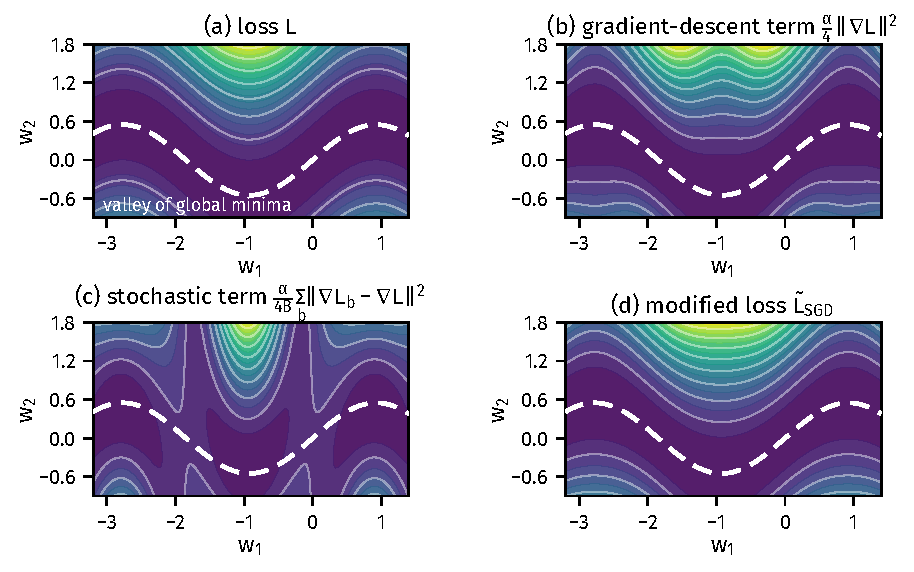
\includegraphics[width=0.67\linewidth]{implicit_sgd}
  \end{center}
  \vspace{-0.75em}
  {\tiny\color{mcMuted}
  (a) the loss. (b) the gradient-descent term, penalising steepness.
  (c) the stochastic term, penalising disagreement between the $B = 12$
  batches. (d) their sum, the modified loss. Both terms vanish on the
  valley floor.
  \hfill Prince (2023), Fig.~9.4.\par}
\end{frame}

\begin{frame}{What this predicts, and what is observed}
  \vspace{0.3em}
  {\scriptsize
  \renewcommand{\arraystretch}{1.42}
  \begin{tabular}{@{}l@{\hspace{1.1em}}l@{\hspace{1.1em}}l@{}}
    \textbf{Change} & \textbf{Effect on the penalty} & \textbf{Observed}\\
    larger step size $\alpha$ & both terms grow, linearly in $\alpha$ &
      full-batch descent generalizes better\\
    smaller batch size & variance term grows as $1/B$ &
      small batches generalize better\\
    momentum, adaptive rates & change the modified loss again &
      the analysis has to be redone\\
  \end{tabular}}
  \vspace{0.85em}

  \begin{itemize}\itemsep0.3em
    \item These are consistent with the analysis but not proved by it:
          the same observations admit other explanations, such as noise
          helping the iterate leave sharp regions
  \end{itemize}
  \srcline{Prince (2023), \S9.2.2 and Fig.~9.5.}
\end{frame}

% =====================================================================
\section{Bias Built Into the Model}
% =====================================================================

\begin{frame}{Invariance and equivariance}
  \vspace{-0.2em}
  \begin{defx}[Invariance and equivariance]\label{th:equi}
    \small
    Let $\mathcal{T}$ be a transformation of the input. A map $\mathcal{C}$ is
    \alert{invariant} under $\mathcal{T}$ if
    $\mathcal{C}(\mathcal{T}(I)) = \mathcal{C}(I)$, and a map $\mathcal{S}$ is
    \alert{equivariant} if
    $\mathcal{S}(\mathcal{T}(I)) = \widetilde{\mathcal{T}}(\mathcal{S}(I))$
    for a corresponding transformation $\widetilde{\mathcal{T}}$ of the
    output. Invariance is the case $\widetilde{\mathcal{T}} = \mathrm{id}$.
  \end{defx}
  \vspace{0.0em}
  {\footnotesize
  \begin{itemize}\itemsep0.20em
    \item Classify an object: translate the image, the label is
          unchanged --- invariance
    \item Segment an object: translate the image, the segmentation
          translates with it --- equivariance
    \item The transformations leaving a property unchanged form a
          \alert{group}: closed, associative, with identity and inverses
  \end{itemize}}
  \srcline{Bishop \& Bishop (2024), Eqs.~9.2--9.4, \S9.1.3--9.1.4.}
\end{frame}

\begin{frame}{Equivariance, on an image}
  \begin{center}
    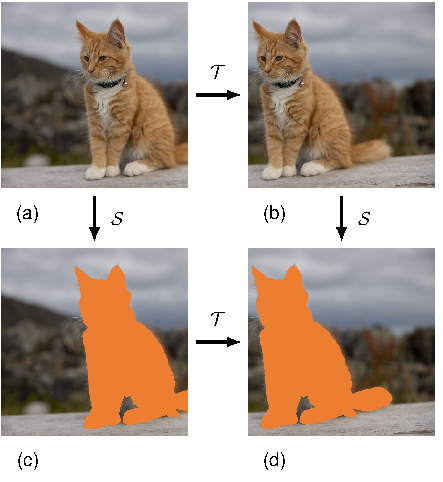
\includegraphics[height=0.56\textheight]{Bishop9_2}
  \end{center}
  \vspace{-0.2em}
  \figcap[0.97]{Translating the image and then segmenting gives the same
  result as segmenting and then translating: the diagram commutes.
  Bishop \& Bishop (2024), Fig.~9.2.}
\end{frame}

\begin{frame}{Equivariance, drawn}
  \vspace{-0.3em}
  \begin{center}
  \begin{tikzpicture}[>=Stealth, font=\scriptsize, scale=1.0,
      im/.style={rounded corners=2pt, draw=shc, line width=1.0pt,
                 minimum width=2.5cm, minimum height=1.7cm,
                 fill=shc!7, align=center},
      ar/.style={->, line width=1.3pt}]
    \node[im] (a) at (0,0)    {image $I$\\[2pt]\tikz\fill[dpc] (0,0) circle (3pt);};
    \node[im] (b) at (5.4,0)  {$\mathcal{T}(I)$\\[2pt]
                               \hspace{1.1cm}\tikz\fill[dpc] (0,0) circle (3pt);};
    \node[im] (c) at (0,-2.7) {$\mathcal{S}(I)$\\[2pt]\tikz\fill[tealc] (0,0) circle (3pt);};
    \node[im] (d) at (5.4,-2.7){$\mathcal{S}(\mathcal{T}(I)) = \mathcal{T}(\mathcal{S}(I))$\\[2pt]
                               \hspace{1.1cm}\tikz\fill[tealc] (0,0) circle (3pt);};

    \draw[ar, dpc]   (a) -- node[above]{$\mathcal{T}$: translate} (b);
    \draw[ar, tealc] (a) -- node[left]{$\mathcal{S}$: segment} (c);
    \draw[ar, tealc] (b) -- node[right]{$\mathcal{S}$} (d);
    \draw[ar, dpc]   (c) -- node[above]{$\mathcal{T}$} (d);

    \node[shc, align=center] at (9.4,-1.35)
      {\textbf{either route}\\ \textbf{gives the same}\\ \textbf{result}};
  \end{tikzpicture}
  \end{center}
  \vspace{-0.45em}
  \begin{itemize}\itemsep0.22em
    \item Building the symmetry into the architecture makes the diagram
          commute by construction, rather than hoping training discovers it
  \end{itemize}
  \srcline{Bishop \& Bishop (2024), Fig.~9.2.}
\end{frame}

\begin{frame}{Four ways to obtain an invariance}
  \vspace{0.3em}
  {\footnotesize
  \renewcommand{\arraystretch}{1.42}
  \begin{tabular}{@{}l@{\hspace{1.1em}}l@{\hspace{1.1em}}l@{}}
    \textbf{Approach} & \textbf{How} & \textbf{Cost}\\
    pre-processing & compute invariant features first &
      may discard useful information\\
    a penalty & punish output change under $\mathcal{T}$ &
      only small transformations\\
    augmentation & train on transformed copies &
      more data, more compute \emph{(Class 19)}\\
    architecture & make the symmetry structural &
      must be known in advance\\
  \end{tabular}}
  \vspace{0.8em}

  \begin{itemize}\itemsep0.3em
    \item Learning the invariance from raw data instead is usually
          hopeless: a shift of a few pixels changes every pixel value,
          and the invariances compose combinatorially
  \end{itemize}
  \srcline{Bishop \& Bishop (2024), \S9.1.3; Simard et al.\ (1992).}
\end{frame}

\begin{frame}{Parameter sharing: a hard constraint}
  \vspace{-0.3em}
  \begin{itemize}\itemsep0.22em
    \item A penalty makes some weights small. \alert{Parameter sharing}
          instead forces groups of weights to be equal, so there are
          fewer degrees of freedom than connections
    \item The shared value is still learned; what is fixed is that the
          group moves together
    \item Backpropagation needs only a small change: the gradient of a
          shared value is the sum of the gradients of its copies, and
          this is how translation equivariance enters a convolutional
          network
    \item \alert{Soft} weight sharing replaces the hard constraint with
          a mixture-of-Gaussians prior, so the groups, their centres and
          spreads are all learned
  \end{itemize}
  \srcline{Bishop \& Bishop (2024), \S9.4--9.4.1; Nowlan \& Hinton (1992).}
\end{frame}

\begin{frame}{Residual connections}
  \vspace{-0.35em}
  \[
    \mathbf{z}_1 = F_1(\mathbf{x}) + \mathbf{x},
    \qquad
    \mathbf{z}_2 = F_2(\mathbf{z}_1) + \mathbf{z}_1,
    \qquad
    \mathbf{y} = F_3(\mathbf{z}_2) + \mathbf{z}_2 .
  \]
  \vspace{-0.5em}
  \begin{center}
  \begin{tikzpicture}[>=Stealth, font=\scriptsize, scale=1.0,
      blk/.style={rounded corners=2pt, draw=shc, fill=shc!10,
                  line width=1.0pt, minimum width=1.15cm,
                  minimum height=0.72cm},
      add/.style={circle, draw=dpc, fill=dpc!12, line width=1.0pt,
                  inner sep=1.6pt},
      ar/.style={->, shc, line width=1.1pt}]
    \node (x) at (0,0) {$\mathbf{x}$};
    \node[blk] (f1) at (1.5,0) {$F_1$};
    \node[add] (a1) at (2.9,0) {$+$};
    \node[blk] (f2) at (4.4,0) {$F_2$};
    \node[add] (a2) at (5.8,0) {$+$};
    \node[blk] (f3) at (7.3,0) {$F_3$};
    \node[add] (a3) at (8.7,0) {$+$};
    \node (y) at (10.0,0) {$\mathbf{y}$};

    \draw[ar] (x) -- (f1); \draw[ar] (f1) -- (a1);
    \draw[ar] (a1) -- node[above]{$\mathbf{z}_1$} (f2);
    \draw[ar] (f2) -- (a2);
    \draw[ar] (a2) -- node[above]{$\mathbf{z}_2$} (f3);
    \draw[ar] (f3) -- (a3); \draw[ar] (a3) -- (y);

    \draw[->, dpc, line width=1.1pt] (0.35,0.32) to[out=55, in=125] (2.9,0.24);
    \draw[->, dpc, line width=1.1pt] (2.9,0.32) to[out=55, in=125] (5.8,0.24);
    \draw[->, dpc, line width=1.1pt] (5.8,0.32) to[out=55, in=125] (8.7,0.24);
  \end{tikzpicture}
  \end{center}
  \vspace{-0.45em}
  \begin{itemize}\itemsep0.22em
    \item Each block learns the \alert{residual}
          $F_l(\mathbf{z}_{l-1}) = \mathbf{z}_l - \mathbf{z}_{l-1}$, so producing the
          identity needs only small parameters
    \item The bias is towards shallow behaviour, with depth available
          when the data pays for it
  \end{itemize}
  \srcline{Bishop \& Bishop (2024), Eqs.~9.35--9.38; He et al.\ (2015).}
\end{frame}

\begin{frame}{Why residual connections smooth the surface}
  \vspace{-0.15em}
  \begin{propx}[A residual network is an ensemble of shallower ones]\label{th:res}
    \small
    Substituting the intermediate variables gives
    \[
      \mathbf{y} = F_3\big(F_2(F_1(\mathbf{x}) + \mathbf{x}) + F_1(\mathbf{x}) + \mathbf{x}\big)
        + F_2\big(F_1(\mathbf{x}) + \mathbf{x}\big) + F_1(\mathbf{x}) + \mathbf{x} ,
    \]
    a sum over every subset of the blocks: paths of depth $3$, $2$, $1$
    and $0$ all in parallel.
  \end{propx}
  \vspace{0.25em}
  \begin{itemize}\itemsep0.26em
    \item The deep path is still there, so nothing is lost in
          representational terms
    \item But the shallow paths have well-behaved gradients, which is
          why the error surface is far less shattered than a plain
          network of the same depth
  \end{itemize}
  \srcline{Bishop \& Bishop (2024), Eq.~9.40, Figs.~9.12, 9.15;
  Balduzzi et al.\ (2017).}
\end{frame}

\begin{frame}{The same network, expanded}
  \vspace{-0.2em}
  \begin{center}
  \begin{tikzpicture}[>=Stealth, font=\scriptsize, x=0.86cm, y=0.84cm,
      blk/.style={rounded corners=2pt, draw=shc, fill=shc!10,
                  line width=0.9pt, minimum width=0.9cm,
                  minimum height=0.52cm},
      add/.style={circle, draw=dpc, fill=dpc!12, line width=0.9pt,
                  inner sep=1.3pt},
      ar/.style={->, shc, line width=0.9pt},
      sk/.style={->, dpc, line width=0.9pt}]
    % rows: 1 (top) to 4 (bottom)
    \foreach \r/\yy in {1/3.3, 2/2.2, 3/1.1, 4/0.0} {
      \node[blk] (f\r) at (2.0,\yy) {$F_1$};
      \node[add] (a\r) at (3.4,\yy) {$+$};
      \draw[ar] (f\r) -- (a\r);
      \draw[ar] (0.7,\yy) -- (f\r);
      \draw[sk] (0.7,\yy-0.42) -- (3.4,\yy-0.42) -- (a\r);
    }
    \node (x) at (0.0,1.65) {$\mathbf{x}$};
    \draw[shc, line width=0.9pt] (x) -- (0.7,1.65);
    \draw[shc, line width=0.9pt] (0.7,-0.42) -- (0.7,3.3);
    % rows 1 and 3 continue through F2
    \foreach \r/\yy in {1/3.3, 3/1.1} {
      \node[blk] (g\r) at (4.8,\yy) {$F_2$};
      \node[add] (b\r) at (6.2,\yy) {$+$};
      \draw[ar] (a\r) -- (g\r);
      \draw[ar] (g\r) -- (b\r);
    }
    % rows 2 and 4 feed the second sum of the row above
    \draw[sk] (a2) -- (6.2,2.2) -- (b1);
    \draw[sk] (a4) -- (6.2,0.0) -- (b3);
    % row 1 continues through F3 to the output sum
    \node[blk] (h1) at (7.6,3.3) {$F_3$};
    \node[add] (out) at (9.0,3.3) {$+$};
    \draw[ar] (b1) -- (h1);
    \draw[ar] (h1) -- (out);
    \draw[sk] (b3) -- (9.0,1.1) -- (out);
    \node (y) at (9.9,3.3) {$\mathbf{y}$};
    \draw[ar] (out) -- (y);
    % labels on the right
    \node[shc, align=left, anchor=west, font=\scriptsize] at (10.3,2.55)
      {$F_3\big(F_2(F_1(\mathbf{x}) + \mathbf{x}) + F_1(\mathbf{x}) + \mathbf{x}\big)$};
    \node[dpc, align=left, anchor=west, font=\scriptsize] at (10.3,0.55)
      {$F_2\big(F_1(\mathbf{x}) + \mathbf{x}\big) + F_1(\mathbf{x}) + \mathbf{x}$};
  \end{tikzpicture}
  \end{center}
  \vspace{-0.3em}
  \figcap[0.97]{The three-block network written out. Every route from
  $\mathbf{x}$ to $\mathbf{y}$ is a network in its own right, from three
  blocks deep to none; the two expressions are the arguments of the
  final addition.}
  \srcline{Bishop \& Bishop (2024), Fig.~9.15.}
\end{frame}

% =====================================================================
\section{Putting It Together}
% =====================================================================

\begin{frame}{What each mechanism prefers}
  \vspace{0.3em}
  {\scriptsize
  \renewcommand{\arraystretch}{1.40}
  \begin{tabular}{@{}l@{\hspace{1.1em}}l@{\hspace{1.1em}}l@{}}
    \textbf{Mechanism} & \textbf{Prefers} & \textbf{Controlled by}\\
    $L^2$ / weight decay & small weights, smooth functions & $\lambda$\\
    lasso, $q = 1$ & few non-zero weights & $\lambda$\\
    layer-wise penalty & the same, respecting rescaling & $\lambda_1, \lambda_2$\\
    gradient descent & flat regions of the surface & step size $\alpha$\\
    stochastic descent & regions where batches agree & batch size $B$\\
    parameter sharing & functions with the chosen symmetry & the grouping\\
    residual connections & shallow behaviour unless paid for & the architecture\\
  \end{tabular}}
  \vspace{0.75em}

  \begin{redhighlight}
    The first three are written into the objective and can be switched
    off. The next two are properties of the optimiser and cannot.
  \end{redhighlight}
\end{frame}

\begin{frame}{Takeaways}
  \vspace{0.1em}
  {\scriptsize
  \begin{enumerate}\itemsep0.34em
    \item Finite data never determines a function, so every learning
          algorithm must prefer some solutions; there is no unbiased
          option (Proposition~\ref{th:nfl})
    \item A penalty on the parameters is a prior over them
          (Proposition~\ref{th:map})
    \item Weight decay suppresses the directions the error function is
          insensitive to, which are the ones fitting noise, and leaves
          the rest nearly alone
    \item A penalty should respect the symmetries of the model, which
          simple weight decay does not (Proposition~\ref{th:consist})
    \item $q = 1$ is the only exponent that is both convex and has
          corners, which is why the lasso is sparse
          (Proposition~\ref{th:lasso})
    \item Gradient descent implicitly minimises
          $L + \tfrac{\alpha}{4}\|\nabla L\|^2$, so the step size is a
          regularization coefficient (Theorem~\ref{th:igd})
    \item Stochastic descent adds the variance of the batch gradients,
          scaling as $1/B$ (Theorem~\ref{th:isgd})
    \item Symmetry, parameter sharing and residual connections put the
          preference in the architecture instead
  \end{enumerate}}
  \bridge{Class 19 turns to what we do to the procedure and the data:
  early stopping, ensembles, dropout and added noise.}
\end{frame}

\begin{frame}[allowframebreaks]{References}
  \vspace{0.3em}
  {\scriptsize
  \begin{enumerate}\itemsep0.30em
    \item C.\ M.\ Bishop \& H.\ Bishop, \emph{Deep Learning: Foundations
          and Concepts}, Springer, 2024. \S9.1 (Eqs.~9.2--9.4,
          Figs.~9.1--9.2); \S9.2 (Eqs.~9.1, 9.5--9.20,
          Figs.~9.3--9.6); \S9.4; \S9.5 (Eqs.~9.32--9.41,
          Figs.~9.12--9.16).
    \item S.\ J.\ D.\ Prince, \emph{Understanding Deep Learning}, MIT
          Press, 2023. \S9.1 (Eqs.~9.1--9.5, Figs.~9.1--9.2);
          \S9.2 (Eqs.~9.6--9.10, Figs.~9.3--9.5).
    \item D.\ H.\ Wolpert, ``The lack of a priori distinctions between
          learning algorithms'', \emph{Neural Computation} 8(7), 1996.
    \item R.\ Tibshirani, ``Regression shrinkage and selection via the
          lasso'', \emph{J.\ Royal Statistical Society B} 58(1), 1996.
    \item P.\ Simard, B.\ Victorri, Y.\ LeCun \& J.\ Denker,
          ``Tangent prop'', NIPS 1992.
    \item S.\ Nowlan \& G.\ E.\ Hinton, ``Simplifying neural networks by
          soft weight sharing'', \emph{Neural Computation} 4(4), 1992.
    \item D.\ G.\ T.\ Barrett \& B.\ Dherin, ``Implicit gradient
          regularization'', ICLR 2021.
    \item S.\ L.\ Smith, B.\ Dherin, D.\ G.\ T.\ Barrett \& S.\ De,
          ``On the origin of implicit regularization in stochastic
          gradient descent'', ICLR 2021.
    \item K.\ He, X.\ Zhang, S.\ Ren \& J.\ Sun, ``Deep residual
          learning for image recognition'', CVPR 2016 (arXiv 2015).
    \item D.\ Balduzzi et al., ``The shattered gradients problem'',
          ICML 2017.
    \item M.\ M.\ Bronstein, J.\ Bruna, T.\ Cohen \& P.\ Veli\v{c}kovi\'c,
          ``Geometric deep learning'', arXiv:2104.13478, 2021.
  \end{enumerate}}
\end{frame}

\begin{frame}[standout]
  Questions?
\end{frame}

\end{document}
